\chapter{Boson hợp thành, biểu diễn spin và sự nhân đôi Dirac}

\section{Đối xứng hoán đổi và boson hợp thành}

Câu hỏi mở đầu là một nghịch lý thực sự về các hạt hợp thành. Nếu hai fermion tạo thành một boson, thì hai boson như vậy có thể chiếm cùng một trạng thái mà không vi phạm nguyên lý loại trừ fermion hay không? Câu trả lời bắt đầu từ chính quy tắc hoán đổi.

Giả sử hai hạt đồng nhất được mô tả bởi một hàm sóng của hai đối số. Các ký hiệu \(x\) và \(y\) gắn nhãn cho hai vị trí hạt; chúng không dùng để phân biệt hai loại hạt khác nhau. Đối với boson thì hàm sóng là đối xứng, còn đối với fermion thì nó phản đối xứng:
\begin{equation}
\Psi_B(x,y)=\Psi_B(y,x),
\qquad
\Psi_F(x,y)=-\Psi_F(y,x).
\end{equation}
Tính đối xứng này nói rằng việc hoán đổi hai hạt không thể phân biệt không tạo ra một trạng thái vật lý mới.

Hai boson chắc chắn có thể cùng chiếm một trạng thái một hạt. Nếu trạng thái đó có hàm sóng \(\varphi\), thì tích hai hạt là
\begin{equation}
\Psi(x,y)=\varphi(x)\varphi(y).
\end{equation}
Hàm sóng là những hàm phức trị thông thường, không phải toán tử hay ma trận, nên các giá trị của chúng giao hoán:
\begin{equation}
\varphi(x)\varphi(y)=\varphi(y)\varphi(x).
\end{equation}
Vì vậy tích này là đối xứng. Cùng cách xây dựng đó không thể cho một trạng thái hai fermion khác không, vì tính phản đối xứng sẽ đòi hỏi
\begin{equation}
\varphi(x)\varphi(y)=-\varphi(y)\varphi(x),
\end{equation}
trong khi hai vế nếu không có dấu trừ thì lại bằng nhau.

Tổng quát hơn, hãy bắt đầu với một hàm sóng hai hạt bất kỳ \(F(x,y)\), không giả thiết trước bất kỳ đối xứng hoán đổi nào. Bỏ qua hệ số chuẩn hóa, phần đối xứng và phần phản đối xứng của nó là
\begin{align}
F_{\mathrm{sym}}(x,y)&=F(x,y)+F(y,x),\\
F_{\mathrm{asym}}(x,y)&=F(x,y)-F(y,x).
\end{align}
Việc kiểm tra dưới phép hoán đổi là tường minh:
\begin{align}
F_{\mathrm{sym}}(y,x)
&=F(y,x)+F(x,y)
=F_{\mathrm{sym}}(x,y),\\
F_{\mathrm{asym}}(y,x)
&=F(y,x)-F(x,y)
=-F_{\mathrm{asym}}(x,y).
\end{align}
Cộng thêm hàm đã hoán đổi thì đối xứng hóa nó; trừ đi hàm đã hoán đổi thì phản đối xứng hóa nó.

Một cặp nguyên tử hiđrô cho trường hợp thú vị hơn. Có bốn fermion cấu thành: hai electron đồng nhất và hai proton đồng nhất. Gọi \(x_1,x_2\) là các biến electron và \(y_1,y_2\) là các biến proton. Hàm sóng bốn vật phải phản đối xứng riêng rẽ dưới phép hoán đổi các electron và dưới phép hoán đổi các proton:
\begin{align}
\Psi(x_2,x_1;y_1,y_2)
&=-\Psi(x_1,x_2;y_1,y_2),\\
\Psi(x_1,x_2;y_2,y_1)
&=-\Psi(x_1,x_2;y_1,y_2).
\end{align}

Để làm rõ động cơ đưa vào hai hàm sóng một nguyên tử phân biệt, hãy hình dung một nguyên tử hiđrô định xứ gần gốc tọa độ, với hàm sóng \(\psi(x,y)\), và một nguyên tử khác định xứ ở nơi khác, với hàm sóng \(\phi(x,y)\). Hàm thứ hai có thể đơn giản chỉ là một bản sao tịnh tiến của hàm thứ nhất, thu được bằng cách tịnh tiến cả đối số electron lẫn đối số proton của nó, nhưng trong thiết lập này nó vẫn là một hàm sóng riêng biệt. Một tích ngây thơ là
\begin{equation}
\psi(x_1,y_1)\phi(x_2,y_2).
\end{equation}
Nó vẫn chưa có bất kỳ tính phản đối xứng fermion bắt buộc nào.

Trước hết, phản đối xứng hóa các biến electron:
\begin{equation}
\Psi_x=
\psi(x_1,y_1)\phi(x_2,y_2)
-\psi(x_2,y_1)\phi(x_1,y_2).
\end{equation}
Dưới \(x_1\leftrightarrow x_2\), hai hạng tử đổi chỗ cho nhau và toàn bộ biểu thức đổi dấu. Bây giờ hãy phản đối xứng hóa kết quả này theo các biến proton. Thứ tự bốn hạng tử được cố định bởi hai bước phản đối xứng hóa liên tiếp.\footnote{Cách xây dựng này cũng cố định mẫu dấu \(+,-,-,+\) thông qua các hiệu chỉnh nhãn biến được thực hiện trong phép tính trình bày bằng lời.}
\begin{align}
\Psi_{2H}(x_1,x_2;y_1,y_2)
&=\Psi_x(x_1,x_2;y_1,y_2)\nonumber\\
&\quad{}-\Psi_x(x_1,x_2;y_2,y_1)\\
&=\psi(x_1,y_1)\phi(x_2,y_2)\nonumber\\
&\quad{}-\psi(x_2,y_1)\phi(x_1,y_2)\nonumber\\
&\quad{}-\psi(x_1,y_2)\phi(x_2,y_1)\nonumber\\
&\quad{}+\psi(x_2,y_2)\phi(x_1,y_1).
\label{eq:two-hydrogen-antisymmetrized}
\end{align}
Một phép hoán đổi electron sẽ hoán đổi hai hạng tử đầu và hai hạng tử cuối, kèm theo sự đảo dấu toàn cục. Một phép hoán đổi proton cũng như vậy. Vì thế trạng thái này có đúng hai tính phản đối xứng riêng rẽ mà các fermion cấu thành đòi hỏi.

\begin{classroomqa}
\lecturetimestamp{00:11:11}
\audiencequestion{Nếu các nguyên tử hiđrô là boson, thì điều gì ngăn cản việc đặt hai nguyên tử chồng trực tiếp lên nhau?}
\lecturerresponse{Thống kê hoán đổi boson không loại bỏ các lực giữa các nguyên tử. Nguyên lý loại trừ Pauli giữa các hạt cấu thành, cùng với các lực liên nguyên tử khác, có thể khiến sự chồng lấp trong không gian trở nên cực kỳ tốn năng lượng. Điều đó khác với việc hỏi liệu các nguyên tử có thể cùng chiếm một trạng thái động lượng phi định xứ hay không. Một trạng thái riêng động lượng trải rộng khắp không gian, nên có cùng động lượng không có nghĩa là ép các nguyên tử vào cùng một điểm. Ngay cả những vật có lõi cứng như các quả bi-a cũng có thể tuân theo thống kê hoán đổi boson: lõi cứng của chúng sẽ ngăn sự chồng lấp trong không gian, trong khi thống kê boson vẫn cho phép cùng chiếm một trạng thái động lượng.}
\end{classroomqa}

\begin{classroomqa}
\lecturetimestamp{00:12:28}
\audiencequestion{Liệu việc đặt hai nguyên tử hiđrô vào cùng một trạng thái riêng động lượng có đặt các fermion cấu thành của chúng vào cùng một trạng thái hay không?}
\lecturerresponse{Không. Trạng thái bốn vật vẫn phản đối xứng dưới phép hoán đổi hai biến electron và, một cách riêng rẽ, phản đối xứng dưới phép hoán đổi hai biến proton. Chỉ có phép hoán đổi đồng thời của cả hai hạt cấu thành---tức là phép hoán đổi hai nguyên tử xét như những toàn thể---mới là đối xứng.}
\end{classroomqa}

Thật vậy, hoán đổi hai nguyên tử nghĩa là thực hiện đồng thời cả hai phép thay thế
\begin{equation}
x_1\leftrightarrow x_2,
\qquad
y_1\leftrightarrow y_2.
\end{equation}
Phép thay thế thứ nhất đóng góp một dấu trừ fermion và phép thứ hai đóng góp thêm một dấu trừ nữa:
\begin{equation}
\begin{aligned}
\Psi_{2H}(x_2,x_1;y_2,y_1)
&=(-1)(-1)\Psi_{2H}(x_1,x_2;y_1,y_2)\\
&=\Psi_{2H}(x_1,x_2;y_1,y_2).
\end{aligned}
\end{equation}
Có thể thấy cùng kết quả đó từng hạng tử một trong phương trình~\eqref{eq:two-hydrogen-antisymmetrized}. Dưới phép hoán đổi toàn nguyên tử,
\begin{equation}
\psi(x_1,y_1)\phi(x_2,y_2)
\longleftrightarrow
\psi(x_2,y_2)\phi(x_1,y_1),
\end{equation}
nên hạng tử thứ nhất và thứ tư hoán đổi cho nhau. Tương tự,
\begin{equation}
-\psi(x_2,y_1)\phi(x_1,y_2)
\longleftrightarrow
-\psi(x_1,y_2)\phi(x_2,y_1),
\end{equation}
nên hạng tử thứ hai và thứ ba hoán đổi cho nhau. Trạng thái đầy đủ là đối xứng dưới phép đổi chỗ các nguyên tử. Hai dấu trừ của các hạt cấu thành cho hạt hợp thành một dấu cộng.

Phát biểu về hoán đổi này độc lập về mặt logic với năng lượng cần để làm các nguyên tử chồng lấp lên nhau. Lực đẩy mạnh có thể khiến sự chồng lấp như vậy không thể đạt tới, nhưng nó không làm thay đổi quy luật hoán đổi đối xứng.

\begin{classroomqa}
\lecturetimestamp{00:14:42}
\audiencequestion{Trạng thái bốn vật đã xây dựng biểu diễn điều gì về mặt vật lý, và nó có phải cụ thể là một trạng thái trong không gian động lượng không?}
\lecturerresponse{Đó là hàm sóng hai nguyên tử thu được từ hai hàm sóng một nguyên tử bằng cách phản đối xứng hóa các nhãn electron rồi đến các nhãn proton. Nó không nhất thiết phải được viết trong không gian động lượng. Các biến có thể mô tả vị trí, động lượng hoặc một biểu diễn khác; các đối xứng hoán đổi bắt buộc của các hạt cấu thành là như nhau.}
\end{classroomqa}

Do đó, hai nguyên tử có thể cùng chiếm một hàm sóng động lượng phi định xứ ngay cả khi việc ép các phân bố không gian của chúng chồng lấp mạnh lên nhau có thể tốn rất nhiều năng lượng.

Bây giờ cho hai hàm sóng một nguyên tử bằng nhau, \(\phi=\psi\). Phương trình~\eqref{eq:two-hydrogen-antisymmetrized} trở thành
\begin{align}
\Psi_{\mathrm{same}}
&=\psi(x_1,y_1)\psi(x_2,y_2)
-\psi(x_2,y_1)\psi(x_1,y_2)\nonumber\\
&\quad
-\psi(x_1,y_2)\psi(x_2,y_1)
+\psi(x_2,y_2)\psi(x_1,y_1).
\end{align}

Trạng thái bốn vật này có triệt tiêu không? Không. Tích thứ nhất và thứ tư bằng nhau, còn tích thứ hai và thứ ba cũng bằng nhau. Dùng tính giao hoán của các hàm sóng một nguyên tử,
\begin{equation}
\Psi_{\mathrm{same}}
=
2\left[
\psi(x_1,y_1)\psi(x_2,y_2)
-\psi(x_2,y_1)\psi(x_1,y_2)
\right],
\label{eq:same-hydrogen-state}
\end{equation}
và biểu thức này nói chung không bằng không. Nó vẫn phản đối xứng theo hai biến electron và, một cách riêng rẽ, phản đối xứng theo hai biến proton.

Ở đây không có sự gán một electron định xứ sắc nét cho mỗi nguyên tử định xứ sắc nét. Một electron liên kết trong nguyên tử là phi định xứ trong không gian theo hàm sóng nguyên tử của nó. Vì vậy, việc cho hai nguyên tử cùng một trạng thái nguyên tử không đồng nghĩa với \(x_1=x_2\), cũng không đồng nghĩa với \(y_1=y_2\).

Nguyên lý loại trừ giữa các hạt cấu thành hiện ra rõ ràng nếu kiểm tra trực tiếp trường hợp trùng nhau. Nếu hai đối số electron được mô hình hóa trùng nhau, \(x_1=x_2=x\), thì phương trình~\eqref{eq:same-hydrogen-state} cho
\begin{align}
\Psi_{\mathrm{same}}(x,x;y_1,y_2)
&=2\bigl[
\psi(x,y_1)\psi(x,y_2)\nonumber\\
&\quad{}-\psi(x,y_1)\psi(x,y_2)
\bigr]\\
&=0.
\end{align}
Biểu thức tương ứng cũng triệt tiêu khi \(y_1=y_2\). Vì vậy, hàm sóng hợp thành ứng với cùng trạng thái không bằng không, trong khi biên độ của nó tại các đối số fermion đồng nhất trùng nhau thì triệt tiêu.\footnote{Spin và mọi nhãn một hạt khác đều bị lược bỏ trong mô hình này. Tính phản đối xứng fermion áp dụng cho tập đầy đủ các nhãn một hạt; sự triệt tiêu được hiển thị ở đây liên quan đến sự trùng nhau của các đối số được giữ lại trong mô hình này.}

\begin{classroomqa}
\lecturetimestamp{00:20:41}
\audiencequestion{Liệu các nguyên tử có thể ở cùng một trạng thái trong khi các electron và proton của chúng lại không ở cùng những trạng thái cấu thành hay không?}
\lecturerresponse{Có. Sự bằng nhau của các hàm sóng nguyên tử hợp thành không loại bỏ các tính phản đối xứng riêng rẽ của electron và proton. Trạng thái bốn vật đầy đủ có thể mô tả hai nguyên tử trong cùng một trạng thái nguyên tử đồng thời gán biên độ bằng không cho các đối số fermion đồng nhất trùng nhau.}
\end{classroomqa}

\begin{classroomqa}
\lecturetimestamp{00:21:12}
\audiencequestion{Phải chăng phép phản đối xứng hóa đã chiếu loại bỏ những phần trong đó các hạt cấu thành đồng nhất trùng nhau?}
\lecturerresponse{Đúng. Trong các biến được hiển thị ở đây, những thành phần trùng nhau đó triệt tiêu chính xác. Phát biểu chính xác là hàm sóng phản đối xứng triệt tiêu khi hai đối số fermion đồng nhất bằng nhau.}
\end{classroomqa}

Sự triệt tiêu này không phụ thuộc vào việc trước hết làm cho các hàm sóng nguyên tử bằng nhau. Với trạng thái tổng quát trong phương trình~\eqref{eq:two-hydrogen-antisymmetrized},
\begin{align}
\Psi_{2H}(x,x;y_1,y_2)
&=\psi(x,y_1)\phi(x,y_2)\nonumber\\
&\quad{}-\psi(x,y_1)\phi(x,y_2)\nonumber\\
&\quad{}-\psi(x,y_2)\phi(x,y_1)\nonumber\\
&\quad{}+\psi(x,y_2)\phi(x,y_1)\\
&=0.
\end{align}

\begin{classroomqa}
\lecturetimestamp{00:21:32}
\audiencequestion{Sự triệt tiêu này có còn đúng khi các nguyên tử ở những trạng thái khác nhau và các biến cấu thành đồng nhất trùng nhau hay không?}
\lecturerresponse{Có. Nó hệ quả từ chính tính phản đối xứng, chứ không phải từ việc đặt \(\phi=\psi\). Cùng phát biểu đó cũng đúng trong một biểu diễn khác: sau khi biến đổi sang không gian động lượng, biên độ sẽ triệt tiêu khi hai đối số động lượng của fermion đồng nhất trùng nhau, miễn là các nhãn một hạt khác đã bị lược bỏ cũng trùng nhau.}
\end{classroomqa}

\section{Spin như một hệ lượng tử hữu hạn chiều}

Toán học của spin lại xuất hiện trong isospin, màu và các đối xứng nội tại khác của vật lý hạt. Sự tương tự này mang tính hình thức: cùng một đại số xuất hiện, mặc dù các đại lượng vật lý không nhất thiết có cùng cách diễn giải. Nhiệm vụ trước mắt là phát triển thêm một chút về spin rồi quay lại phương trình Dirac. Bộ công cụ này về sau sẽ được dùng cho isospin, một khái niệm về mặt lịch sử gắn với thập niên 1930.

Electron là một hạt spin-\(\tfrac12\), cũng như proton và muon. Thành phần \(z\) của spin của nó có hai giá trị khả dĩ. Trước khi chọn đơn vị, ta viết
\begin{equation}
S_z=m\hbar.
\end{equation}
Từ đây về sau \(\hbar=1\). Ký hiệu \(L\) theo quy ước được dành cho mômen động lượng quỹ đạo, nên spin nội tại sẽ được ký hiệu là \(S\). Nó thỏa mãn cùng một đại số mômen động lượng:
\begin{equation}
[S_x,S_y]=iS_z,
\quad
[S_y,S_z]=iS_x,
\quad
[S_z,S_x]=iS_y,
\end{equation}
và
\begin{equation}
S_\pm=S_x\pm iS_y.
\end{equation}
Toán tử \(S_+\) nâng giá trị riêng của \(S_z\) và \(S_-\) hạ nó.

\begin{classroomqa}
\lecturetimestamp{00:25:39}
\audiencequestion{Ở đây thảo luận có nhắm riêng vào spin nội tại không?}
\lecturerresponse{Trọng tâm dự định là spin nội tại. Cùng đại số mômen động lượng đó còn áp dụng tổng quát hơn, kể cả cho mômen động lượng quỹ đạo hoặc sự quay của một vật vĩ mô.}
\end{classroomqa}

Đối với spin một phần hai, các giá trị riêng duy nhất của \(S_z\) là \(+\tfrac12\) và \(-\tfrac12\). Tạm thời gác sang một bên mọi điều khác về electron: quên vị trí và động lượng của nó đi, chỉ giữ lại hai trạng thái spin. Khi đó
\begin{equation}
|\psi\rangle
=
\alpha|\uparrow_z\rangle+\beta|\downarrow_z\rangle
\quad\longleftrightarrow\quad
\begin{pmatrix}
\alpha\\
\beta
\end{pmatrix},
\end{equation}
trong đó
\begin{equation}
|\alpha|^2=P(\uparrow_z),
\qquad
|\beta|^2=P(\downarrow_z),
\qquad
|\alpha|^2+|\beta|^2=1.
\end{equation}
Đây là một không gian trạng thái hai chiều. Điều này không phải là một khẳng định rằng không gian thông thường có hai chiều.

\begin{classroomqa}
\lecturetimestamp{00:28:18}
\audiencequestion{Có phải đã nói rằng không gian vật lý là hai chiều không?}
\lecturerresponse{Không. Không gian trạng thái spin là hai chiều. Vị trí và động lượng đã tạm thời bị lược bỏ, như thể electron bị đóng đinh vào tường và chỉ có spin của nó mới có thể được đo.}
\end{classroomqa}

Các toán tử trên không gian trạng thái này được biểu diễn bởi các ma trận \(2\times2\). Thuận tiện là chọn cơ sở \(S_z\) sao cho \(S_z\) có dạng chéo, nhưng tính chéo là một lựa chọn cơ sở chứ không phải một yêu cầu vật lý.

\begin{classroomqa}
\lecturetimestamp{00:29:46}
\audiencequestion{\(S_z\) có nhất thiết phải có dạng chéo không?}
\lecturerresponse{Không. Nó được chọn có dạng chéo chỉ vì thuận tiện. Các biểu diễn ma trận khác vẫn tương đương về mặt vật lý.}
\end{classroomqa}

\begin{classroomqa}
\lecturetimestamp{00:30:08}
\audiencequestion{\(S_z\) có phải là một ma trận không?}
\lecturerresponse{\(S_z\) là một đại lượng quan sát được và vì thế là một toán tử. Trong cơ sở hữu hạn chiều đã chọn, toán tử đó được biểu diễn bởi một ma trận tác dụng lên các vectơ trạng thái.}
\end{classroomqa}

Một biểu diễn đặc biệt hữu ích là
\begin{equation}
S_i=\frac12\sigma_i,
\end{equation}
trong đó
\begin{equation}
\sigma_x=
\begin{pmatrix}
0&1\\
1&0
\end{pmatrix},
\quad
\sigma_y=
\begin{pmatrix}
0&-i\\
i&0
\end{pmatrix},
\quad
\sigma_z=
\begin{pmatrix}
1&0\\
0&-1
\end{pmatrix}.
\end{equation}
Các ma trận không có thừa số một phần hai là các ma trận Pauli; bản thân các toán tử spin thì có kèm thừa số đó. Phép nhân trực tiếp xác nhận các hệ thức giao hoán. Biểu diễn này không duy nhất: quay các trục hoặc đổi cơ sở sẽ cho một bộ ba tương đương khác.

Đây là một biểu diễn hai thành phần của mômen động lượng spin một phần hai.

\subsection{Các trạng thái riêng dọc theo các trục tọa độ}

Việc giải các phương trình giá trị riêng theo từng thành phần là hữu ích. Vì các giá trị riêng của \(\sigma_i\) là \(\pm1\), nên các giá trị riêng của \(S_i=\sigma_i/2\) là \(\pm\tfrac12\).

Đối với \(\sigma_z\), hai phương trình là
\begin{align}
\begin{pmatrix}
1&0\\
0&-1
\end{pmatrix}
\begin{pmatrix}
\alpha\\
\beta
\end{pmatrix}
&=
\begin{pmatrix}
\alpha\\
\beta
\end{pmatrix},
&
\begin{pmatrix}
1&0\\
0&-1
\end{pmatrix}
\begin{pmatrix}
\alpha\\
\beta
\end{pmatrix}
&=
-
\begin{pmatrix}
\alpha\\
\beta
\end{pmatrix}.
\end{align}

\begin{figure}[t]
\centering
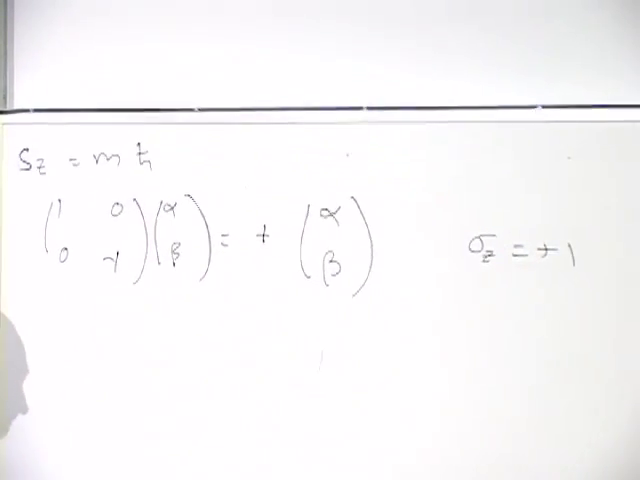
\includegraphics[width=0.74\textwidth]{lecture_08_figure_02.png}
\caption{Phương trình giá trị riêng \(+1\) của \(\sigma_z\) tác dụng lên một spinor hai thành phần.}
\lectureframe{00:34:57}
\end{figure}

Với trị riêng \(+1\), phép nhân theo từng hàng cho
\begin{equation}
\begin{pmatrix}
1\cdot\alpha+0\cdot\beta\\
0\cdot\alpha-\beta
\end{pmatrix}
=
\begin{pmatrix}
\alpha\\
-\beta
\end{pmatrix}
=
\begin{pmatrix}
\alpha\\
\beta
\end{pmatrix}.
\end{equation}
Phương trình trên tự động thỏa mãn, còn phương trình dưới cho \(-\beta=\beta\), do đó \(\beta=0\). Điều kiện chuẩn hóa đòi hỏi \(|\alpha|=1\); chọn pha tổng thể không quan trọng sao cho \(\alpha=1\),
\begin{equation}
|+z\rangle=
\begin{pmatrix}
1\\
0
\end{pmatrix}.
\end{equation}

Với trị riêng \(-1\),
\begin{equation}
\begin{pmatrix}
\alpha\\
-\beta
\end{pmatrix}
=
\begin{pmatrix}
-\alpha\\
-\beta
\end{pmatrix}.
\end{equation}
Bây giờ phương trình dưới tự động thỏa mãn, còn phương trình trên cho \(\alpha=-\alpha\), nên \(\alpha=0\). Chọn \(\beta=1\) ta được
\begin{equation}
|-z\rangle=
\begin{pmatrix}
0\\
1
\end{pmatrix}.
\end{equation}

Bây giờ hãy đổi thí nghiệm và đo \(S_x\). Vì
\begin{equation}
\sigma_x
\begin{pmatrix}
\alpha\\
\beta
\end{pmatrix}
=
\begin{pmatrix}
0\cdot\alpha+\beta\\
\alpha+0\cdot\beta
\end{pmatrix}
=
\begin{pmatrix}
\beta\\
\alpha
\end{pmatrix},
\end{equation}
phương trình \(+1\) trở thành
\begin{equation}
\begin{pmatrix}
\beta\\
\alpha
\end{pmatrix}
=
\begin{pmatrix}
\alpha\\
\beta
\end{pmatrix}.
\end{equation}
Hai phương trình theo thành phần, \(\beta=\alpha\) và \(\alpha=\beta\), là cùng một điều kiện. Chuẩn hóa cho
\begin{equation}
2|\alpha|^2=1,
\end{equation}
nên một lựa chọn thuận tiện là
\begin{equation}
|+x\rangle
=
\frac{1}{\sqrt2}
\begin{pmatrix}
1\\
1
\end{pmatrix}.
\end{equation}

\begin{figure}[t]
\centering
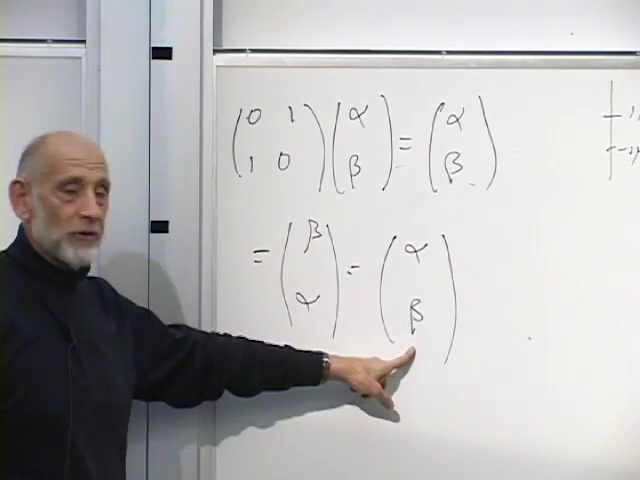
\includegraphics[width=0.74\textwidth]{lecture_08_figure_03.png}
\caption{Với trị riêng \(+1\), \(\sigma_x\) hoán đổi hai thành phần, nên cần \(\alpha=\beta\).}
\lectureframe{00:39:42}
\end{figure}

\begin{classroomqa}
\lecturetimestamp{00:40:13}
\audiencequestion{Nếu bao gồm hệ số một phần hai, thì trị riêng có phải là một phần hai không?}
\lecturerresponse{Có. Ma trận Pauli \(\sigma_x\) có các trị riêng \(\pm1\), còn \(S_x=\sigma_x/2\) có các trị riêng \(\pm\tfrac12\).}
\end{classroomqa}

Với trị riêng \(-1\),
\begin{equation}
\begin{pmatrix}
\beta\\
\alpha
\end{pmatrix}
=
-
\begin{pmatrix}
\alpha\\
\beta
\end{pmatrix},
\end{equation}
nên
\begin{equation}
\beta=-\alpha,
\qquad
\alpha=-\beta.
\end{equation}
Đây lại là cùng một phương trình. Sau khi chuẩn hóa,
\begin{equation}
|-x\rangle
=
\frac{1}{\sqrt2}
\begin{pmatrix}
1\\
-1
\end{pmatrix}.
\end{equation}
Vì vậy, một chồng chập với hệ số bằng nhau của spin lên theo \(z\) và spin xuống theo \(z\) được phân cực dọc theo trục \(x\) dương, còn trạng thái cùng dạng với một dấu trừ tương đối thì được phân cực dọc theo trục \(x\) âm.

Đối với hướng \(y\),
\begin{equation}
\sigma_y
\begin{pmatrix}
\alpha\\
\beta
\end{pmatrix}
=
\begin{pmatrix}
-i\beta\\
i\alpha
\end{pmatrix}.
\end{equation}
Hai vectơ riêng đã chuẩn hóa là
\begin{equation}
|+y\rangle
=
\frac{1}{\sqrt2}
\begin{pmatrix}
1\\
i
\end{pmatrix},
\qquad
|-y\rangle
=
\frac{1}{\sqrt2}
\begin{pmatrix}
1\\
-i
\end{pmatrix},
\end{equation}
trừ một pha tổng thể. Cả hai trạng thái đều cho xác suất \(1/2\) đối với spin lên theo \(z\) và \(1/2\) đối với spin xuống theo \(z\). Pha tương đối \(i\), vốn không lộ ra trong hai xác suất đó, phân biệt sự phân cực theo \(y\) với sự phân cực theo \(x\). Các tổ hợp tuyến tính cũng mô tả spin phân cực theo những hướng tùy ý; phép tính ấy được để lại sau.

\begin{classroomqa}
\lecturetimestamp{00:44:22}
\audiencequestion{Dấu của thành phần \(i\) có phải đã được gán cho sai trị riêng của \(\sigma_y\) không?}
\lecturerresponse{Quả thật dấu ấy có thể đã được gán cho sai trị riêng. Ở đây việc gán còn chưa chắc chắn; nó không được ấn định theo trí nhớ.}
\end{classroomqa}

Phép kiểm tra trực tiếp là
\begin{align}
\sigma_y\frac{1}{\sqrt2}
\begin{pmatrix}
1\\
i
\end{pmatrix}
&=
\frac{1}{\sqrt2}
\begin{pmatrix}
-i\,i\\
i
\end{pmatrix}
=
\frac{1}{\sqrt2}
\begin{pmatrix}
1\\
i
\end{pmatrix},\\
\sigma_y\frac{1}{\sqrt2}
\begin{pmatrix}
1\\
-i
\end{pmatrix}
&=
\frac{1}{\sqrt2}
\begin{pmatrix}
(-i)(-i)\\
i
\end{pmatrix}
=
-\frac{1}{\sqrt2}
\begin{pmatrix}
1\\
-i
\end{pmatrix}.
\end{align}
Vì vậy \(+i\) thuộc về trị riêng \(+1\), còn \(-i\) thuộc về trị riêng \(-1\).\footnote{Cách gán được nói miệng vẫn chưa ngã ngũ sau vài lần đảo ngược; các dấu trình bày ở đây được cố định bởi phép nhân ma trận đã hiển thị.} Mọi trạng thái spin 1/2, kể cả mọi trạng thái phân cực theo một hướng tùy ý, đều là tổ hợp tuyến tính của \(|+z\rangle\) và \(|-z\rangle\).

\section{Spin 1 và spinor phụ thuộc vị trí}

Đối với spin \(1\), các giá trị có thể có của \(S_z\) là \(+1,0,-1\). Vì thế không gian trạng thái là ba chiều. Spin \(1\) là spin nguyên và tương ứng với thống kê boson. Ta tìm ba ma trận \(3\times3\) thỏa mãn cùng các hệ thức giao hoán của mômen góc.

Một biểu diễn đối xứng giữa ba hướng tọa độ được cho dưới đây.\footnote{Dấu của \(S_y\) theo ma trận nhìn thấy gần \(00{:}48{:}50\), và cũng được cố định bởi \([S_x,S_y]=iS_z\). Đảo dấu đó sẽ đảo ngược giao hoán tử cần có.}
\begin{equation}
\begin{aligned}
S_x
&=
i
\begin{pmatrix}
0&0&0\\
0&0&1\\
0&-1&0
\end{pmatrix},
&
S_y
&=
i
\begin{pmatrix}
0&0&1\\
0&0&0\\
-1&0&0
\end{pmatrix},\\
S_z
&=
i
\begin{pmatrix}
0&1&0\\
-1&0&0\\
0&0&0
\end{pmatrix}.
\end{aligned}
\end{equation}
Mỗi ma trận là \(i\) nhân với một ma trận phản đối xứng thực. Mỗi ma trận chứa một \(1\), một \(-1\), và một hàng cùng một cột triệt tiêu gắn với chính tọa độ của nó: hàng-cột thứ nhất cho \(S_x\), thứ hai cho \(S_y\), và thứ ba cho \(S_z\). Điều này cho một mẹo ghi nhớ hữu ích. Trong biểu diễn này \(S_z\) không ở dạng đường chéo.

Đặt
\begin{equation}
v=
\begin{pmatrix}
\alpha\\
\beta\\
\gamma
\end{pmatrix}.
\end{equation}
Khi đó
\begin{equation}
S_zv
=
\begin{pmatrix}
i\beta\\
-i\alpha\\
0
\end{pmatrix}.
\end{equation}
Với trị riêng \(+1\),
\begin{equation}
i\beta=\alpha,
\qquad
-i\alpha=\beta,
\qquad
0=\gamma.
\end{equation}
Suy ra \(\beta=-i\alpha\) và \(\gamma=0\). Chuẩn hóa cho \(2|\alpha|^2=1\), nên
\begin{equation}
|m=+1\rangle
=
\frac{1}{\sqrt2}
\begin{pmatrix}
1\\
-i\\
0
\end{pmatrix}.
\end{equation}
Với trị riêng \(-1\),
\begin{equation}
i\beta=-\alpha,
\qquad
-i\alpha=-\beta,
\qquad
0=-\gamma,
\end{equation}
do đó \(\beta=i\alpha\), \(\gamma=0\), và
\begin{equation}
|m=-1\rangle
=
\frac{1}{\sqrt2}
\begin{pmatrix}
1\\
i\\
0
\end{pmatrix}.
\end{equation}
Cuối cùng, phương trình trị riêng bằng 0 cho \(\alpha=\beta=0\), để \(\gamma\) tùy ý. Nghiệm chuẩn hóa của nó là
\begin{equation}
|m=0\rangle
=
\begin{pmatrix}
0\\
0\\
1
\end{pmatrix}.
\end{equation}
Không còn trị riêng nào khác: ba vectơ riêng này bao hết không gian ba chiều. Các hệ số \(1/\sqrt2\) không phải chỉ để cho đẹp. Về sau chính các hệ số ấy sẽ đi vào các dự đoán thực nghiệm định lượng khi đại số được áp dụng cho isospin.

\begin{classroomqa}
\lecturetimestamp{00:54:10}
\audiencequestion{Nên đọc các phần tử phức của những vectơ riêng spin 1 này như thế nào?}
\lecturerresponse{Với \(m=+1\) các thành phần là \(1/\sqrt2,-i/\sqrt2,0\); với \(m=-1\) chúng là \(1/\sqrt2,i/\sqrt2,0\); và với \(m=0\) chúng là \(0,0,1\).}
\end{classroomqa}

Những bộ ba ma trận khác cũng thỏa mãn cùng đại số và tương đương về mặt vật lý. Biểu diễn đối xứng ở trên hữu ích vì ba hướng được đối xử như nhau, và nó sẽ còn được dùng lại.

\subsection{Khôi phục vị trí}

Bây giờ ta xét lại chuyển động của hạt. Spin giao hoán với vị trí và với xung lượng, nên có thể chỉ định một trong hai cùng với một thành phần spin. Vị trí và xung lượng không giao hoán, và các thành phần spin khác nhau cũng không giao hoán với nhau.

Một hạt spin 1/2 đang chuyển động được mô tả bởi một spinor phụ thuộc vị trí,
\begin{equation}
\psi(x)=
\begin{pmatrix}
\psi_\uparrow(x)\\
\psi_\downarrow(x)
\end{pmatrix}.
\end{equation}
Các đại lượng
\begin{equation}
\rho_{\uparrow_z}(x)=|\psi_\uparrow(x)|^2,
\qquad
\rho_{\downarrow_z}(x)=|\psi_\downarrow(x)|^2
\end{equation}
là các mật độ xác suất đồng thời của vị trí và spin. Tổng của chúng,
\begin{equation}
\rho(x)=\psi^\dagger(x)\psi(x)
=|\psi_\uparrow(x)|^2+|\psi_\downarrow(x)|^2,
\end{equation}
là mật độ vị trí. Nếu biết hạt đã được phát hiện tại \(x\), thì các xác suất có điều kiện là
\begin{equation}
P(\uparrow_z\mid x)
=
\frac{|\psi_\uparrow(x)|^2}{\psi^\dagger(x)\psi(x)},
\qquad
P(\downarrow_z\mid x)
=
\frac{|\psi_\downarrow(x)|^2}{\psi^\dagger(x)\psi(x)},
\end{equation}
miễn là \(\rho(x)\neq0\). Vì vậy một electron được biểu diễn bởi một hàm sóng không gian hai thành phần, trong đó các biên độ spin cục bộ được phép biến thiên từ nơi này sang nơi khác.

Đối với một hạt spin 1 đang chuyển động, viết
\begin{equation}
\phi(x)=
\begin{pmatrix}
\phi_1(x)\\
\phi_2(x)\\
\phi_3(x)
\end{pmatrix}.
\end{equation}
Tại mỗi điểm trong không gian, ba thành phần tạo thành một vectơ trong cùng không gian spin đã dùng ở trên. Các hạt spin 1 có spin nguyên và là boson.

\begin{classroomqa}
\lecturetimestamp{01:00:10}
\audiencequestion{Bản thân \(\phi_1(x)\) có phải là xác suất cho kết quả spin 1 \(m=+1\) không?}
\lecturerresponse{Không. Nó là một biên độ trong cơ sở ba thành phần đã chọn. Để thu được một kết quả spin xác định, hãy lập bra của vectơ riêng chuẩn hóa tương ứng, chiếu trường lên nó, rồi lấy bình phương môđun.}
\end{classroomqa}

\begin{figure}[t]
\centering
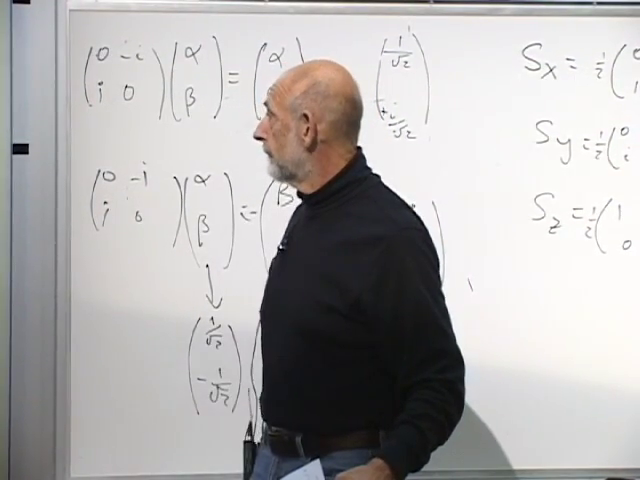
\includegraphics[width=0.82\textwidth]{lecture_08_figure_04.png}
\caption{Các vectơ riêng đã chuẩn hóa của \(\sigma_y\) cùng với ba ma trận spin 1/2.}
\lectureframe{01:00:12}
\end{figure}

Ví dụ,
\begin{equation}
\begin{aligned}
|m=+1\rangle
&=
\frac{1}{\sqrt2}
\begin{pmatrix}
1\\
-i\\
0
\end{pmatrix}
\\
\Longrightarrow\quad\langle m=+1|
&=
\frac{1}{\sqrt2}
\begin{pmatrix}
1&i&0
\end{pmatrix}.
\end{aligned}
\end{equation}
Vì thế biên độ chiếu là
\begin{align}
\langle m=+1|\phi(x)\rangle
&=
\frac{1}{\sqrt2}
\begin{pmatrix}
1&i&0
\end{pmatrix}
\begin{pmatrix}
\phi_1(x)\\
\phi_2(x)\\
\phi_3(x)
\end{pmatrix}\\
&=
\frac{\phi_1(x)+i\phi_2(x)}{\sqrt2}.
\end{align}
Áp dụng cùng quy tắc ấy cho cả ba vectơ riêng cho ta các mật độ phân giải theo spin.\footnote{Các công thức này hoàn tất đại số chiếu sau khi đã đính chính tường minh rằng \(\phi_1\) và \(\phi_2\) không nhất thiết phải là số thực. Nếu coi chúng là thực thì sẽ xóa nhầm sự giao thoa phân biệt các mật độ \(m=+1\) và \(m=-1\).}
\begin{align}
\rho_{+1}(x)
&=
\frac12\left|\phi_1(x)+i\phi_2(x)\right|^2,\\
\rho_{-1}(x)
&=
\frac12\left|\phi_1(x)-i\phi_2(x)\right|^2,\\
\rho_0(x)
&=
|\phi_3(x)|^2.
\end{align}
Chúng thỏa mãn
\begin{equation}
\begin{aligned}
\rho_{+1}(x)+\rho_{-1}(x)+\rho_0(x)
&=
|\phi_1(x)|^2+|\phi_2(x)|^2
\\
&\quad{}+|\phi_3(x)|^2
\\
&=
\phi^\dagger(x)\phi(x).
\end{aligned}
\end{equation}
Nếu điều kiện là hạt đã được phát hiện tại \(x\), thì
\begin{equation}
P(m\mid x)
=
\frac{\rho_m(x)}{\phi^\dagger(x)\phi(x)},
\end{equation}
miễn là \(\phi^\dagger(x)\phi(x)\neq0\). Quy tắc đo tổng quát luôn như nhau: lập bra của vectơ riêng chuẩn hóa mong muốn, chiếu trạng thái thực tế lên nó, rồi lấy bình phương môđun. Mật độ thu được vẫn giữ sự phụ thuộc vào vị trí.

Các ma trận spin cao hơn phức tạp hơn, nhưng nguyên lý không thay đổi.

\begin{classroomqa}
\lecturetimestamp{01:07:31}
\audiencequestion{Không gian trạng thái lớn đến mức nào đối với spin 3/2?}
\lecturerresponse{Nó có bốn trạng thái, với \(m=\tfrac32,\tfrac12,-\tfrac12,-\tfrac32\). Spin 2 có năm trạng thái.}
\end{classroomqa}

\begin{classroomqa}
\lecturetimestamp{01:07:55}
\audiencequestion{Vì sao phần trình bày có \(x,y,z\) mà không có hướng thời gian nào? Cách xử lý này có phải là phi tương đối tính không?}
\lecturerresponse{Cho đến đây thì là phi tương đối tính. Spin, cũng như khối lượng, được đặc trưng đơn giản nhất trong hệ quy chiếu nghỉ của hạt; mô tả của nó trong một hệ quy chiếu quán tính khác thu được bằng phép biến đổi Lorentz thích hợp. Bước tương đối tính đó được để lại sau.}
\end{classroomqa}

Phương trình Dirac cung cấp bối cảnh tương đối tính và giải thích vì sao hàm sóng bốn thành phần của nó chứa một bộ đôi spin.

\section{Các ma trận Dirac và spinor bốn thành phần}

Hàm sóng Dirac bốn thành phần thỏa mãn
\begin{equation}
i\frac{\partial\Psi}{\partial t}
=
-i\alpha_i\frac{\partial\Psi}{\partial x_i}
+m\beta\Psi,
\qquad i=1,2,3,
\end{equation}
trong đó một chỉ số không gian lặp lại thì được quy ước lấy tổng. Vì thế số hạng đạo hàm có nghĩa là
\begin{equation}
\alpha_1\frac{\partial\Psi}{\partial x}
+\alpha_2\frac{\partial\Psi}{\partial y}
+\alpha_3\frac{\partial\Psi}{\partial z}.
\end{equation}
Đối với một sóng phẳng, điều này trở thành phương trình đại số
\begin{equation}
\omega\Psi=(\alpha_i k_i+m\beta)\Psi.
\end{equation}

\begin{classroomqa}
\lecturetimestamp{01:11:32}
\audiencequestion{Hai lần xuất hiện của \(m\) có ký hiệu cùng một thứ không?}
\lecturerresponse{Không. Một cái đang được dùng làm chỉ số không gian, còn cái kia là khối lượng của hạt. Hãy đổi tên chỉ số không gian thành \(i\); khi \(i\) xuất hiện hai lần thì nó được lấy tổng từ \(1\) đến \(3\).}
\end{classroomqa}

Khi bình phương, toán tử tần số phải tái tạo hệ thức tương đối tính
\begin{equation}
\omega^2=\mathbf{k}^2+m^2.
\end{equation}
Do đó, các hạng bình phương đòi hỏi, với mỗi \(i\),
\begin{equation}
\alpha_i^2=I_4,
\qquad
\beta^2=I_4.
\end{equation}

\begin{classroomqa}
\lecturetimestamp{01:13:01}
\audiencequestion{\(\beta\) có khác nhau đối với từng thành phần trong bốn thành phần của \(\Psi\) không?}
\lecturerresponse{Không. Chỉ có một ma trận \(\beta\), tác dụng lên toàn bộ spinor bốn thành phần, và nó thỏa mãn \(\beta^2=I_4\).}
\end{classroomqa}

Các hạng chéo phải triệt tiêu. Đối với những hướng không gian khác nhau, và cả giữa mọi \(\alpha_i\) và \(\beta\), ta có
\begin{equation}
\alpha_i\alpha_j+\alpha_j\alpha_i=0
\quad (i\neq j),
\qquad
\alpha_i\beta+\beta\alpha_i=0.
\end{equation}
Tương đương,
\begin{equation}
\{\alpha_i,\alpha_j\}=2\delta_{ij}I_4,
\quad
\{\alpha_i,\beta\}=0,
\quad
\{\beta,\beta\}=2I_4.
\end{equation}
Mỗi ma trận phản giao hoán với mọi ma trận khác nó, còn phản giao hoán tử của nó với chính nó bằng hai lần ma trận đơn vị.

Nếu không có \(\beta\), thì ba ma trận Pauli đã cung cấp sẵn ba ma trận \(2\times2\) bình phương lên cho ma trận đơn vị và phản giao hoán từng đôi. Hạng khối lượng đòi hỏi một ma trận thứ tư như vậy. Không có ma trận \(2\times2\) thứ tư nào có các tính chất cần thiết, và các ma trận \(3\times3\) cũng không thỏa mãn đại số này. Vì vậy biểu diễn nhỏ nhất là \(4\times4\).

Một ma trận \(4\times4\) có thể được chia thành bốn khối \(2\times2\). Trong một biểu diễn thuận tiện,
\begin{equation}
\alpha_i=
\begin{pmatrix}
\sigma_i&0\\
0&-\sigma_i
\end{pmatrix},
\qquad i=1,2,3.
\end{equation}

\begin{figure}[t]
\centering
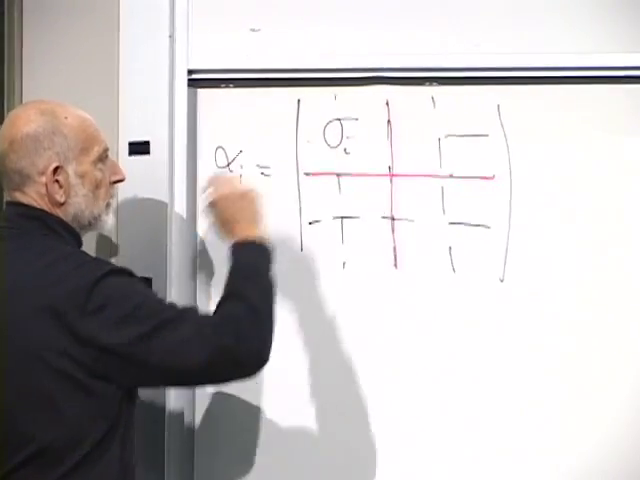
\includegraphics[width=0.68\textwidth]{lecture_08_figure_05.png}
\caption{Ma trận Dirac \(\alpha_i\) được viết thành các khối \(2\times2\), với \(\sigma_i\) và \(-\sigma_i\) trên đường chéo.}
\lectureframe{01:17:23}
\end{figure}

\begin{classroomqa}
\lecturetimestamp{01:17:41}
\audiencequestion{Trong biểu diễn trước đó, các khối \(\sigma_i\) có được sắp xếp theo cách ngược lại không?}
\lecturerresponse{Có. Trong một biểu diễn khác, chúng được đặt ngoài đường chéo. Hai cách sắp xếp là tương đương và liên hệ với nhau bằng một phép biến đổi đồng dạng.}
\end{classroomqa}

Trong biểu diễn hiện tại, ma trận còn lại là
\begin{equation}
\beta=
\begin{pmatrix}
0&I_2\\
I_2&0
\end{pmatrix},
\qquad
I_2=
\begin{pmatrix}
1&0\\
0&1
\end{pmatrix}.
\end{equation}
Phép nhân theo khối rút việc kiểm tra đại số \(4\times4\) về phép nhân thông thường của các ma trận \(2\times2\).

\begin{classroomqa}
\lecturetimestamp{01:19:17}
\audiencequestion{Biểu diễn trước đó có dùng một dấu khác hoặc một dạng chéo cho \(\beta\) không?}
\lecturerresponse{Nó dùng một cơ sở khác nhưng tương đương về mặt vật lý. Một phép đổi cơ sở trộn bốn thành phần của \(\Psi\) và làm thay đổi hình thức của các ma trận mà không làm thay đổi vật lý.}
\end{classroomqa}

Bốn phần tử của \(\Psi\) không phải là bốn tọa độ của không-thời gian. Chúng là các tọa độ trong không gian vectơ nhỏ nhất mà trên đó đại số phản giao hoán này có thể tác dụng. Có hai cấu trúc phân đôi phân biệt: sự chia thành các khối \(2\times2\) và cấu trúc Pauli hai thành phần bên trong mỗi khối. Đón trước cách diễn giải sẽ được thiết lập ở dưới, bốn khả năng có thể được sắp xếp thành
\begin{equation}
\begin{array}{c|cc}
& S_z=+\tfrac12 & S_z=-\tfrac12\\ \hline
\omega>0 & (\omega>0,+\tfrac12) & (\omega>0,-\tfrac12)\\
\omega<0 & (\omega<0,+\tfrac12) & (\omega<0,-\tfrac12)
\end{array}.
\end{equation}
Hàng dưới gồm các trạng thái electron tần số âm. Nó không phải là một hàng positron; positron sẽ được diễn giải như một lỗ trống trong tập đã lấp đầy của các trạng thái ấy.

\section{Sự nhân đôi năng lượng trong hệ nghỉ và positron}

Cấu trúc năng lượng hai nhánh bộc lộ rõ nhất tại xung lượng bằng 0. Khi \(\mathbf{k}=0\), trạng thái sóng phẳng là hằng theo không gian và số hạng đạo hàm theo không gian biến mất. Phương trình trong hệ nghỉ\footnote{Khung hình tại \(01{:}23{:}38\) vẫn còn tạm thời một hệ số \(i\) thừa ở hạng khối lượng; lời đính chính bằng lời tại \(01{:}24{:}05\) loại bỏ nó.} là
\begin{equation}
i\frac{\partial\Psi}{\partial t}=m\beta\Psi.
\end{equation}

\begin{figure}[t]
\centering
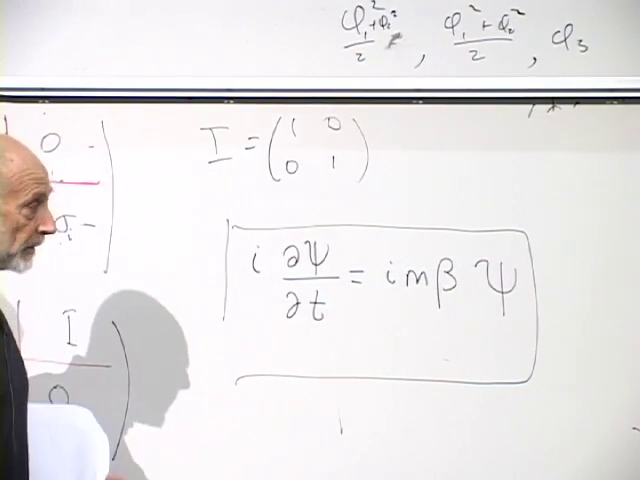
\includegraphics[width=0.76\textwidth]{lecture_08_figure_06.png}
\caption{Tại xung lượng bằng 0, các đạo hàm theo không gian triệt tiêu, để lại phương trình đã hiệu chỉnh trong hệ nghỉ \(i\partial_t\Psi=m\beta\Psi\).}
\lectureframe{01:23:38}
\end{figure}

Tách cột bốn thành phần thành một đối tượng hai thành phần ở trên và một đối tượng hai thành phần ở dưới:
\begin{equation}
\Psi=
\begin{pmatrix}
\psi_+\\
\psi_-
\end{pmatrix}.
\end{equation}

\begin{classroomqa}
\lecturetimestamp{01:24:47}
\audiencequestion{Các nhãn \(\psi_+\) và \(\psi_-\) đã có nghĩa là năng lượng dương và năng lượng âm chưa?}
\lecturerresponse{Chưa. Ở giai đoạn này, chúng chỉ là tên gọi cho các khối hai thành phần ở trên và ở dưới. Các tổ hợp năng lượng của chúng vẫn chưa được tìm ra.}
\end{classroomqa}

\begin{classroomqa}
\lecturetimestamp{01:25:10}
\audiencequestion{Vectơ cột bốn thành phần được chia đôi này biểu diễn cái gì?}
\lecturerresponse{Đó vẫn là cùng một spinor Dirac bốn thành phần, được sắp xếp cho khớp với dạng khối của các ma trận. Mỗi nửa là một đối tượng hai thành phần, và hai đối tượng như vậy hợp thành vectơ cột bốn thành phần ban đầu.}
\end{classroomqa}

Ma trận \(\beta\) hoán đổi hai khối:
\begin{equation}
\beta
\begin{pmatrix}
\psi_+\\
\psi_-
\end{pmatrix}
=
\begin{pmatrix}
\psi_-\\
\psi_+
\end{pmatrix}.
\end{equation}
Vì thế, phương trình trong hệ nghỉ trở thành
\begin{equation}
i\frac{\partial\psi_+}{\partial t}=m\psi_-,
\qquad
i\frac{\partial\psi_-}{\partial t}=m\psi_+.
\end{equation}

Có hai gợi ý tự nhiên. Lấy thêm một đạo hàm theo thời gian sẽ khử ghép hệ, nhưng lấy tổng và hiệu của hai phương trình thì chéo hóa chúng ngay lập tức. Thật vậy,
\begin{align}
i\frac{\partial}{\partial t}(\psi_++\psi_-)
&=m(\psi_++\psi_-),\\
i\frac{\partial}{\partial t}(\psi_+-\psi_-)
&=-m(\psi_+-\psi_-).
\end{align}
Đặt
\begin{equation}
\chi_+=\psi_++\psi_-,
\qquad
\chi_-=\psi_+-\psi_-,
\end{equation}
ta được hai phương trình độc lập,
\begin{equation}
i\partial_t\chi_+=m\chi_+,
\qquad
i\partial_t\chi_-=-m\chi_-.
\end{equation}
Với sự phụ thuộc theo tần số xác định \(e^{-i\omega t}\), tổng có
\begin{equation}
\omega=+m,
\end{equation}
trong khi hiệu có
\begin{equation}
\omega=-m.
\end{equation}
Đây chính là sự nhân đôi năng lượng dương và năng lượng âm đã thấy trong ví dụ một chiều trước đó: phương trình tương đối tính lại có các nghiệm electron năng lượng dương và năng lượng âm. Vì thế, sự nhân đôi theo khối tách thành các nhánh năng lượng dương và năng lượng âm. Các trạng thái thuần trong hệ nghỉ có thể được viết
\begin{equation}
\Psi_{\omega=+m}=
\begin{pmatrix}
\xi\\
\xi
\end{pmatrix},
\qquad
\Psi_{\omega=-m}=
\begin{pmatrix}
\xi\\
-\xi
\end{pmatrix},
\end{equation}
trong đó \(\xi\) vẫn là một đối tượng hai thành phần tùy ý.

Tổng và hiệu đã loại bỏ một cấu trúc bội hai, nhưng hai thành phần của \(\xi\) vẫn còn. Các ma trận Pauli tác dụng lên cặp còn lại này. Đây là cặp gắn với spin, như sẽ được kiểm tra bằng lập luận về phép quay và định luật bảo toàn ở dưới.

\begin{classroomqa}
\lecturetimestamp{01:32:23}
\audiencequestion{Có thể coi spin là cấu trúc bội hai ở ngoài và dấu năng lượng là cấu trúc bội hai ở trong không?}
\lecturerresponse{Có. Hai cách sắp thứ tự các thừa số là tương đương. Ta có thể hoán đổi chỉ số nào được viết trước; sự thay đổi ấy chỉ là sự xáo lại của bốn thành phần.}
\end{classroomqa}

Nhánh tần số âm dẫn tới cách diễn giải biển Dirac. Một tần số âm được gán cho năng lượng electron âm. Lấp đầy mọi trạng thái electron năng lượng âm sẽ hạ năng lượng xuống thấp nhất mà nguyên lý loại trừ cho phép, vì mỗi trạng thái fermion hoàn chỉnh chỉ có thể bị chiếm bởi một electron. Khi đó, biển năng lượng âm được lấp đầy hoàn toàn được gọi là chân không.

Nâng một electron từ biển đã lấp đầy này lên một trạng thái năng lượng dương. Kết quả chứa một electron năng lượng dương và một trạng thái năng lượng âm không bị chiếm. Lấy đi một năng lượng âm làm tăng năng lượng, nên lỗ trống có năng lượng kích thích dương; vì thiếu một electron nên nó cũng mang điện tích ngược dấu. Lỗ trống ấy là positron.

\begin{classroomqa}
\lecturetimestamp{01:32:57}
\audiencequestion{Có thể giải thích lại một lần nữa cách diễn giải về positron không?}
\lecturerresponse{Tổng của hai khối có tần số dương còn hiệu có tần số âm. Các nghiệm tần số âm là các trạng thái electron năng lượng âm, và chân không thu được bằng cách lấp đầy tất cả chúng. Nâng một electron đã bị chiếm lên năng lượng dương để lại đồng thời một electron năng lượng dương và một lỗ trống. Lỗ trống mang năng lượng dương và điện tích ngược dấu đó chính là positron.}
\end{classroomqa}

Vì vậy, phép đại số này đồng thời cho ra hai hệ quả: các nhánh năng lượng dương và âm, vốn trở thành cấu trúc hạt--phản hạt, và một cấu trúc hai thành phần còn lại gắn với spin một phần hai. Điểm nổi bật là cả hai đều xuất hiện từ những ma trận nhỏ nhất có thể thỏa mãn các quan hệ phản giao hoán tương đối tính. Vào thời điểm spin mới chỉ vừa xuất hiện như một tính chất thực nghiệm, cấu trúc toán học này lại tạo ra các hạt có spin đồng thời với một nhánh phản hạt; trong bối cảnh lịch sử ấy, kết quả đó là một điều gây chấn động.

\begin{classroomqa}
\lecturetimestamp{01:35:14}
\audiencequestion{Bản thân các electron năng lượng âm có phải là positron không?}
\lecturerresponse{Không. Các trạng thái electron năng lượng âm được lấp đầy trong chân không. Một positron là sự vắng mặt của một electron trong tập đã lấp đầy đó: một lỗ trống, không phải một electron năng lượng âm.}
\end{classroomqa}

Một lỗ trống có thể tham gia vào các chuyển dời. Một positron có năng lượng dương vì nó là sự vắng mặt của một electron năng lượng âm. Nếu một electron năng lượng dương lấp lỗ trống, electron và positron sẽ hủy nhau, nhưng năng lượng của chúng phải được mang đi, thông thường bởi các photon. Theo ngôn ngữ biển, một electron đã lấp vào một trạng thái năng lượng âm chưa bị chiếm. Cùng sự giải phóng năng lượng đó cũng có thể được hình dung như một electron kích thích trong nguyên tử rơi xuống mức thấp hơn: chuyển dời đi xuống phát ra các photon.

\begin{classroomqa}
\lecturetimestamp{01:36:39}
\audiencequestion{Tại sao các electron năng lượng âm ở mức cao hơn không rơi vào lỗ trống?}
\lecturerresponse{Câu hỏi đó trộn lẫn hai trường hợp. Một electron năng lượng dương lấp lỗ trống là sự hủy cặp electron--positron, trong đó các photon mang năng lượng đi. Một chuyển dời của một electron trong biển năng lượng âm là một quá trình khác, sẽ được xét ở dưới.}
\end{classroomqa}

Bản thân phép tính tại động lượng bằng không đã xác lập một suy biến bội hai sau khi dấu năng lượng được tách ra. Một suy biến của hai trạng thái, tự nó, không phải là bằng chứng rằng các trạng thái ấy mang mômen góc.

\begin{classroomqa}
\lecturetimestamp{01:37:44}
\audiencequestion{Làm thế nào phép tính tại động lượng bằng không chứng minh rằng cặp trạng thái còn lại là spin?}
\lecturerresponse{Cặp đó có thể được gọi là lên và xuống, và các ma trận Pauli xuất hiện trong phương trình đầy đủ, nhưng chỉ riêng điều đó vẫn chưa phải là chứng minh. Cần chỉ ra cặp ấy biến đổi thế nào dưới các phép quay trong không gian, hoặc việc gán cho nó spin làm cho tổng mômen góc được bảo toàn trong các tương tác và va chạm. Phần chứng minh ấy được hoãn lại.}
\end{classroomqa}

Đối với một trạng thái nghỉ năng lượng dương, khối trên và khối dưới bằng nhau,
\begin{equation}
\Psi_{\omega=+m}=
\begin{pmatrix}
\xi\\
\xi
\end{pmatrix}.
\end{equation}
Việc xác lập rằng \(\xi\) là một doublet mômen góc đòi hỏi lập luận về phép quay hoặc bảo toàn vừa mô tả; điều đó không suy ra chỉ từ việc đếm hai thành phần.

\begin{classroomqa}
\lecturetimestamp{01:40:46}
\audiencequestion{Một electron khác có thể hủy với positron ngay cả khi năng lượng của nó khác không?}
\lecturerresponse{Có. Các electron không giữ danh tính cá thể. Bất kỳ electron sẵn có nào cũng có thể lấp lỗ trống, và những khác biệt về năng lượng và động lượng ban đầu được phản ánh trong số lượng cũng như năng lượng của các photon phát ra.}
\end{classroomqa}

Bức tranh lỗ trống cũng giải thích một chuyển dời hoàn toàn bên trong biển năng lượng âm. Giả sử một trạng thái năng lượng âm đang bị chiếm chuyển vào lỗ trống. Lỗ trống ban đầu được lấp đầy, nhưng trạng thái mà electron ấy xuất phát từ đó nay lại trống. Lỗ trống đã di chuyển. Tương đương, positron đã đổi năng lượng của nó và đã phát ra bức xạ.

\begin{classroomqa}
\lecturetimestamp{01:42:12}
\audiencequestion{Tại sao các mức năng lượng âm lân cận không thể lần lượt rơi vào lỗ trống?}
\lecturerresponse{Chúng có thể làm cho lỗ trống chuyển từ mức này sang mức khác. Một electron rơi vào lỗ trống cũ để lại một lỗ trống mới tại năng lượng trước đó của nó, nên positron ban đầu trở thành một positron có năng lượng khác. Hiệu năng lượng được các photon mang đi.}
\end{classroomqa}

\begin{classroomqa}
\lecturetimestamp{01:44:39}
\audiencequestion{Tại sao điều này không tạo ra một chuỗi bức xạ đi xuống vô tận?}
\lecturerresponse{Vì năng lượng và động lượng phải được bảo toàn đồng thời. Hai định luật bảo toàn đó không cho phép quá trình không bị ràng buộc này. Cùng vấn đề ấy cũng nảy sinh đối với một electron tự do thông thường: nó không thể cứ đơn giản tiếp tục hạ năng lượng của mình bằng cách phát các photon trong không gian trống.}
\end{classroomqa}